\chapter{\leavevmode\newline Research background}
\chaptermark{Heading on Chapter Pages}
\label{chap:chapter3}

In the past decade, advancements in sensor and hardware capabilities have brought the concept of autonomous vehicles closer to realization. The popularity of events including the DARPA Grand Challenges \parencite{buehler20072005}\parencite{buehler2009darpa} has motivated major automotive companies and tech companies to further develop self-driving technology and deploy such technologies in daily life scenario. The potential benefits of eliminating human intervention in driving are manifold, which aims to enhance road safety, reduce traffic congestion, decrease carbon emissions, and offer mobility to those unable to drive. It represents a shift towards sustainable and efficient transportation, potentially transforming urban planning, energy consumption, and societal accessibility. Such technological strides not only offer car companies an opportunity to differentiate themselves in a competitive market but also align with the increasing demands of the transportation sector. With transportation being a significant contributor to global carbon emissions, regulatory bodies such as the European Road Transport Research Advisory Council and the European Commission have delineated ambitious targets. Their vision is to achieve a $50 \%$ enhancement in transport efficiency by 2030, relative to 2010, and simultaneously curtail emissions by $60 \%$. 

Nowadays, Advanced Driver Assistance System (ADAS) has been developed to enhance road safety by aiding drivers in maintaining vehicle stability, and has emerged as a bridge between today's vehicles and the future of full autonomy. While classical perception, path planning, and motion control methods can handle the majority of driving scenarios, there remain certain corner cases where these traditional techniques fails. These complex and often unpredictable scenarios present unique challenges that cannot be easily resolved using conventional approaches. As a result, the modern ADAS algorithm integrates various sensors and algorithms to assist drivers, making driving safer and more efficient. From simple parking assistance to complex adaptive cruise control, these systems represent the intersection of robotics, artificial intelligence, and vehicular engineering and try to create more sustainable, efficient, and safer transportation solutions.

Compared with vehicles which does not have additonal trailer connected to the ego vehicle body, the truck-trailer wheeled robot, have always brought challenges to the classical state estimation and control methods. While there has been significant progress in developing state and parameter estimation techniques for single-unit vehicles, the area of vehicle-trailer system state and parameter estimation still can be explored, and especially when considering the task of reverse driving. The dynamics involved in reversing a truck-trailer system differ significantly from those of forward driving, primarily due to the inherent instability and non-holonomic constraints (constraints that are non-integrable into positional constraints) of the system. When a truck attempts to reverse with a trailer, the angle between the truck and trailer can quickly grow uncontrollable, leading to a phenomenon known as jack-knifing.

In the previous research, control of such systems was the domain of skilled human operators; however, with the advent of automation and the push towards autonomous vehicles to wider user scenario, there has been a growing interest in developing algorithms that can reliably and safely control truck-trailer systems during reverse driving. Traditional control methods, such as Proportional-Integral-Derivative (PID) controllers, Linear Quadratic Regulators (LQR), and Model Predictive Control (MPC), have been explored for this purpose. While these methods have seen success, they often rely on accurate models of the system dynamics and can struggle with the nonlinearities and uncertainties from the real-world driving scenarios. In recent times, methods that take advantage of modern machine learning techniques, such as deep reinforcement learning , have been introduced, which combines the capabilities of deep learning for recognizing complex patterns with reinforcement learning for decision-making. This fusion enables systems to learn and adapt through continuous interaction with complex environment and adjust its strategy to achieve optimal control.

\section{Overview of path planning}

Historically, path planning was primarily based on geometric and grid-based methods. Geometric methods, such as the Voronoi diagram, partitioned the workspace into regions to find the safest path. Grid-based methods, on the other hand, divided the environment into a grid and used search algorithms to find the path. However, these methods often faced challenges in complex environments or when high precision was required. One of the most popular methods used in autonomous parking is Dubins curve, which is named after Lester Eli Dubins, is a mathematical solution that provides the shortest curve between two points in the plane with a constraint on the curvature. While the Dubins Curve itself was introduced in the 1950s, and with an assumption that the vehicle traveling the path can only travel forward. If the vehicle can also travel in reverse, then the path follows the Reeds–Shepp curve \parencite{reeds1990optimal}, its application to automated parking has been a more recent development, and its integration into parking algorithms allowed for smooth and efficient paths that adhered to the nonholonomic constraints of vehicles, such as a fixed minimum turning radius.

\begin{figure}[h]
\centering
\resizebox{\textwidth}{!}{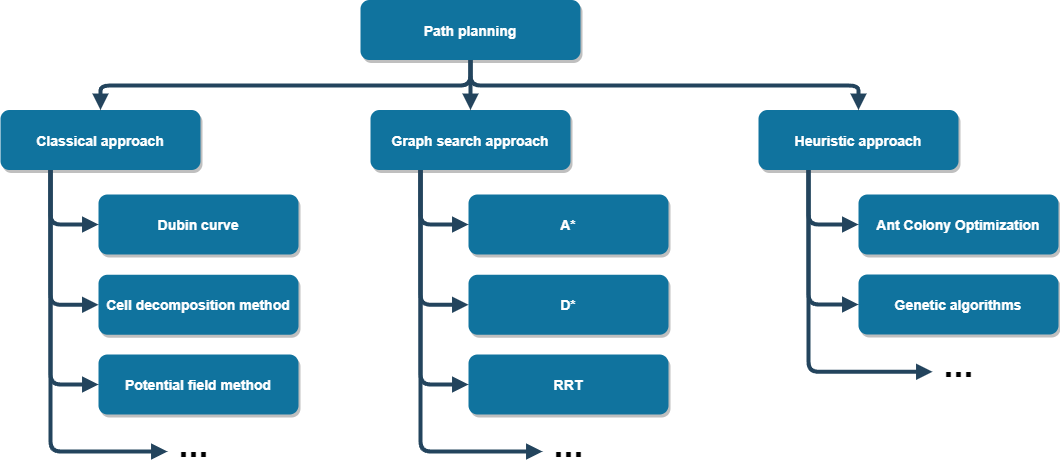
\includegraphics{fig/path_planning_map.png}}
\caption{Map of path planning methods}
\label{fig: path planning map}
\end{figure}

Nowadays, graph search algorithms are becoming dominantly popular and are fundamental to path planning, as they provide systematic ways to explore and navigate through a network of nodes and edges representing the environment. The most basic graph search algorith is Dijkstra algorithm \parencite{dijkstra2022note}, and it has been a foundational method commonly used in applications like Google Maps, known for its guaranteed optimal solutions but criticized for its computational intensity in blind searches. However, the computational-intensity limits the Dijkstra’s blind searches capability, and as a result A* \parencite{hart1968formal} and its variants are becoming the state of the art algorithms for use within static environments, they combined the benefits of both, using a heuristic to guide the search towards the goal while also considering the actual cost from the start. A* guarantees to find the shortest path if an admissible and consistent heuristic is used, and by using a heuristic that estimates the cost to the goal, A* often explores fewer nodes than algorithms like Dijkstra's, making it more efficient in many cases. The A* algorithm and its variants are a significant milestone in the field of path planning, because the balance between efficiency and optimal helped the industry to reduce cost and improve stability.

However, A* and A* re-planner are used for shortest path evaluation based on the information regarding the obstacles present in the environment, and the shortest path evaluation for the known static environment is a two-level problem, which comprises a selection of feasible node pairs and shortest path evaluation based on the obtained feasible node pairs \parencite{dudi2020shortest}. Both of the above mentioned criteria are not available in a dynamic environment, which makes the algorithm inefficient and impractical in dynamic environments. To support path planning in dynamic environments, D* \parencite{stentz1994optimal} and its variants are discussed as efficient tools for quick re-planning in cluttered environments. As D* and its variants do not guarantee solution quality in large dynamic environments, we also explore Rapidly-exploring Random Trees (RRTs) \parencite{lavalle1998rapidly} and a hybrid approach combining Relaxed A* ( RA*) \parencite{ammar2016relaxed} and one meta-heuristic algorithm. The hybrid approach comprises two phases: the initialization of the algorithm using RA* and a post-optimization phase using one heuristic method that improves the quality of solution found in the previous phase. Three meta-heuristic algorithms are also discussed: namely, the Genetic, Ant colony, and Firefly algorithms. These are aimed at providing effective features in pursuit of a hybrid approach to path planning.

The A* algorithm, although effective in static environments, its application in dynamic settings is hindered by its two-level problem structure, involving the selection of feasible node pairs and path evaluation based on these pairs. This makes A* less practical in ever-changing environments. To address the challenges in dynamic environments, incremental versions of A* such as the D* algorithm have been developed, allowing for path updates as new information becomes available1. However, D* and its derivatives may not always ensure solution quality in extensive dynamic landscapes \parencite{stentz1994optimal}. D* is designed to handle changes in the environment, allowing for efficient replanning without having to restart the search from scratch, and it is able to reuse the previous computations, and efficiently update the solution when changes occur, making it suitable for real-time applications. However, D* and its derivatives may not always ensure solution quality in extensive dynamic landscapes, and as result, A rapidly exploring random tree (RRT) is designed to efficiently search nonconvex, high-dimensional spaces by randomly building a space-filling tree. 

Path planning is a critical aspect of autonomous driving and ADAS, guiding the ego vehicle go through complex environments. Algorithms like Dubins curve, Dijkstra's, A*, RRT, and D* are chosen as they represent different facets of path planning, serving as various scenarios from static to dynamic environments, and from deterministic to probabilistic approaches. The trend of integrating AI, particularly machine learning, into path planning is reshaping the field. By leveraging data-driven insights and adaptive algorithms, AI-enhanced path planning offers the potential for more robust, efficient, and intelligent navigation. This fusion of traditional algorithms with AI techniques signifies a promising direction for future innovation and optimization in path planning \parencite{mcmahon2022survey}.

\section{Overview of vehicle control}

The evolution of control theory in autonomous driving and Advanced Driver Assistance Systems (ADAS) has been marked by the development and application of various control strategies, reflecting the complexity and diversity of the challenges in this field. 

\begin{figure}[h]
\centering
\resizebox{\textwidth}{!}{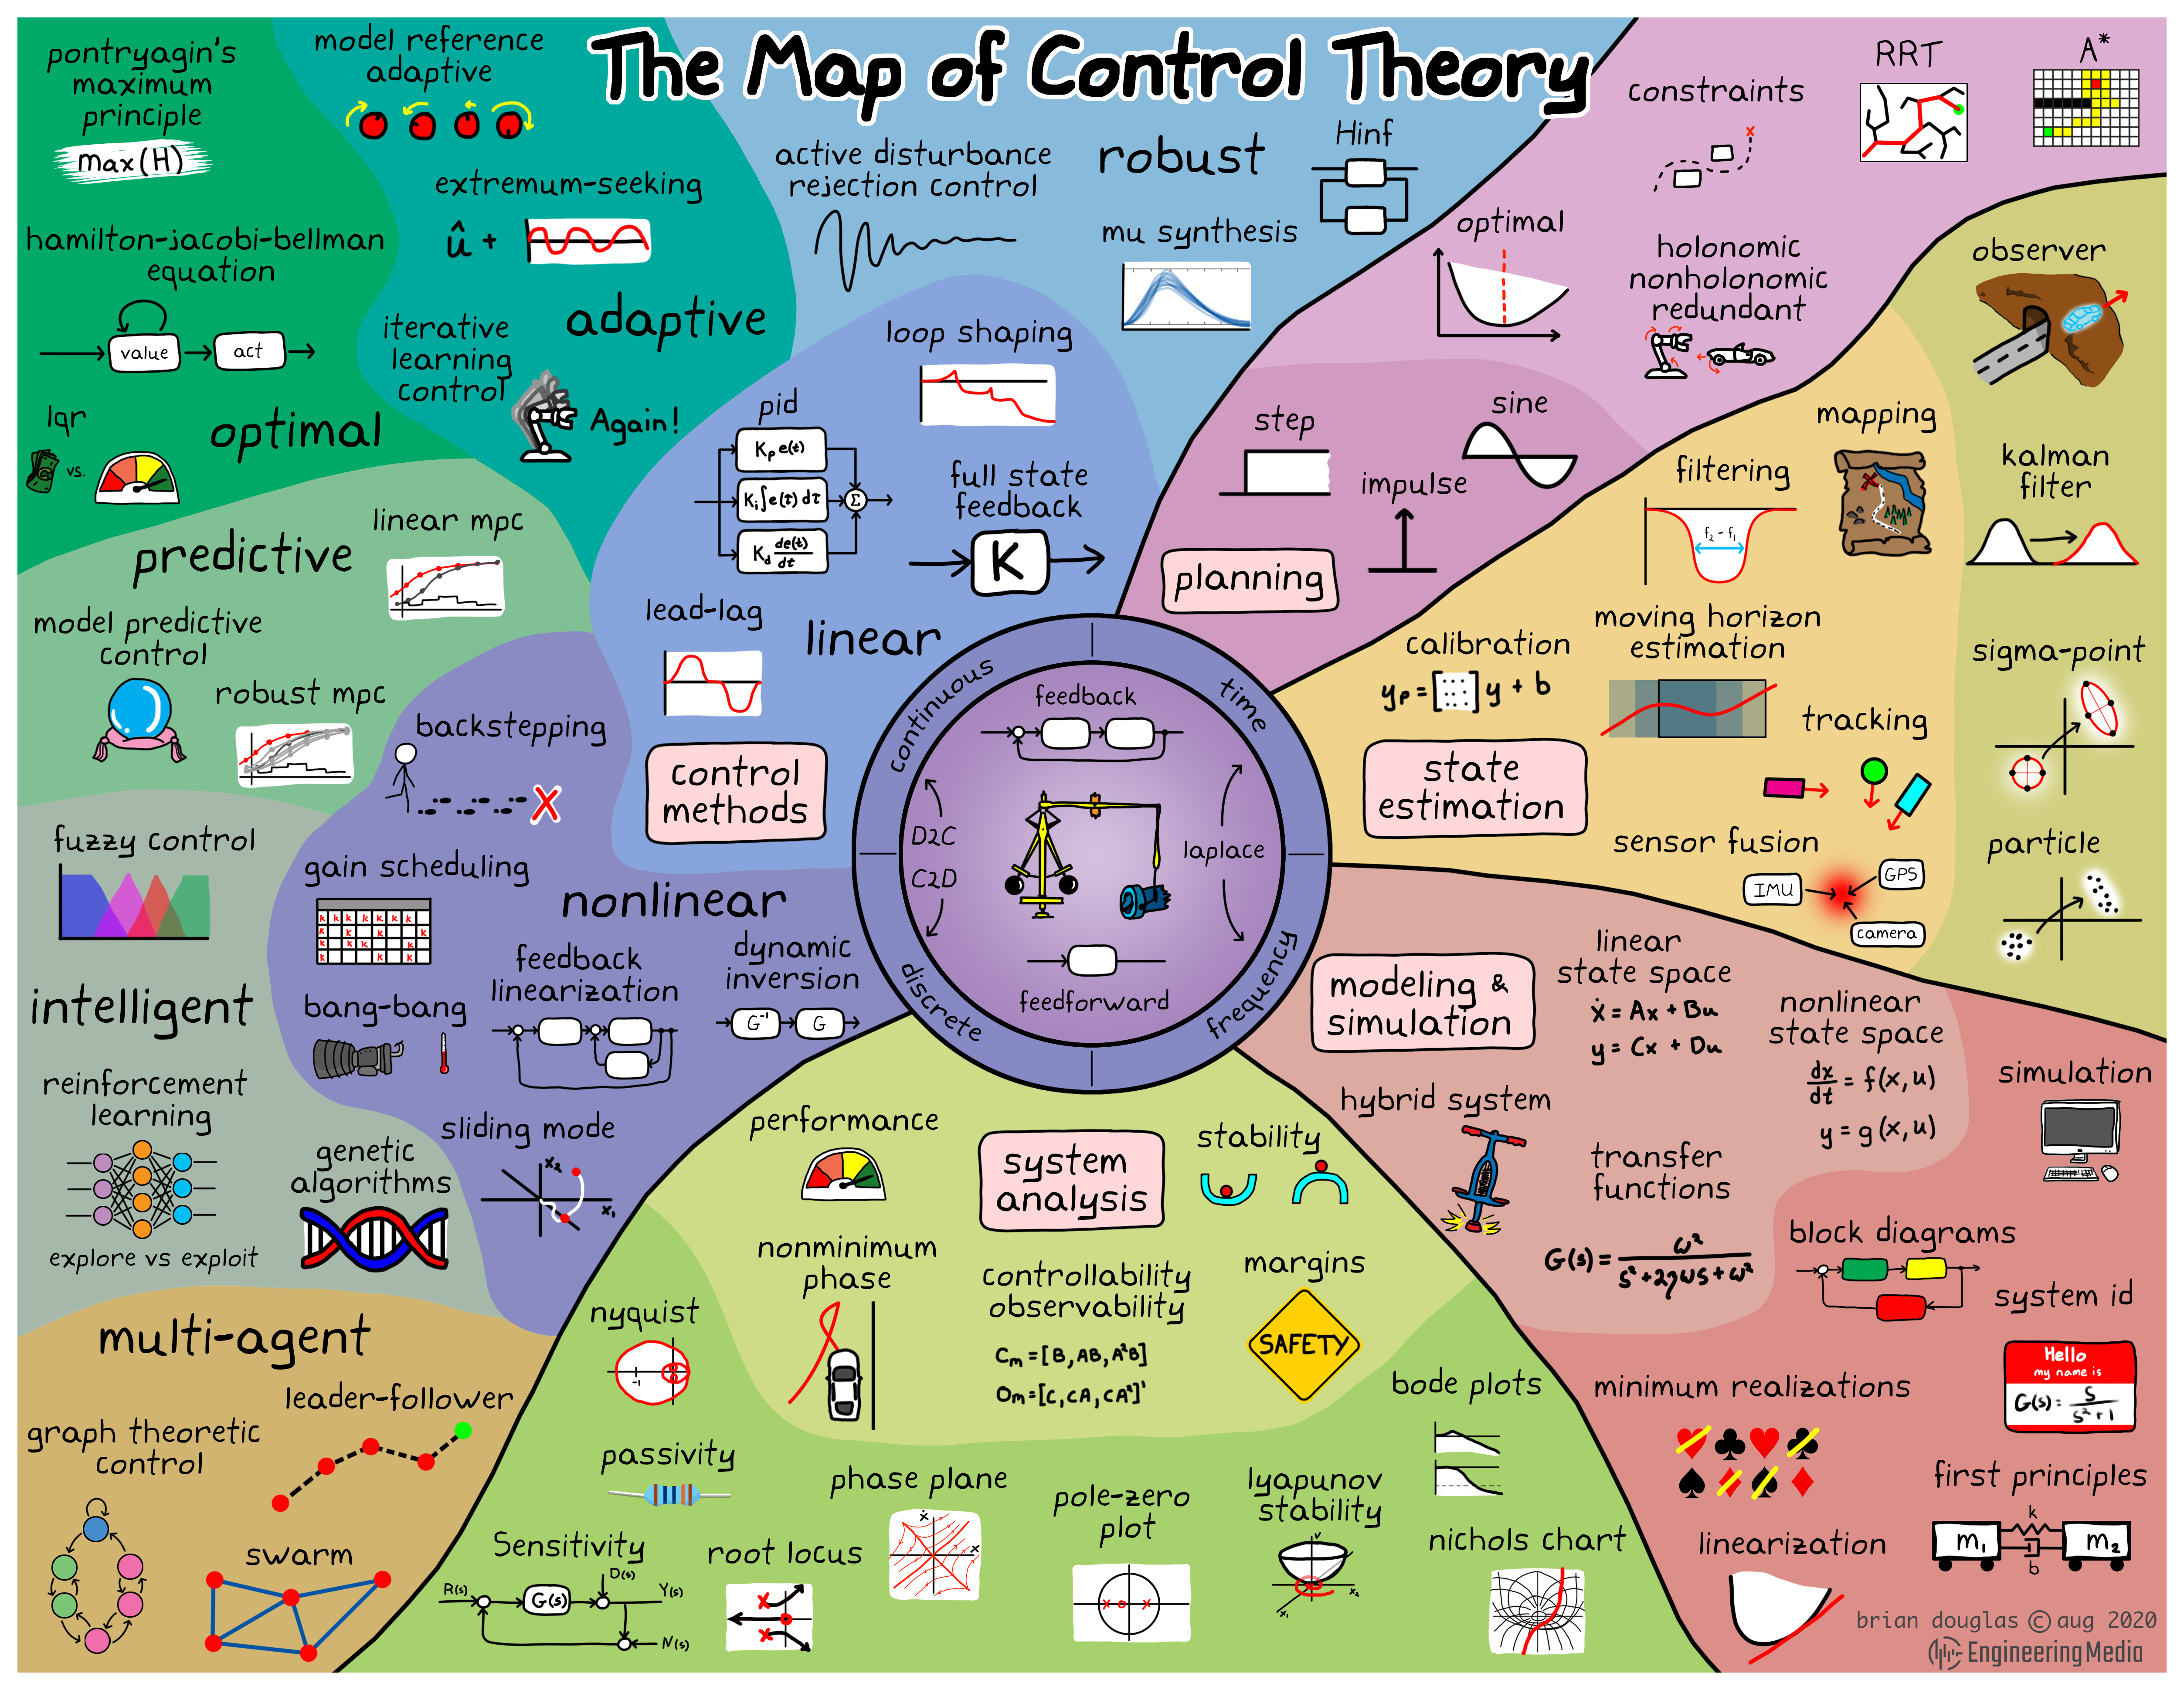
\includegraphics{fig/Control_Map_ver5.png}}
\caption{Map of control theory\parencite{EngineeringMedia}}
\label{fig: control map}
\end{figure}

Starting with PID control, which originated in the early 1920s, initially applied to automatic steering systems for ships. This marked the first theoretical analysis and practical utilization of PID in a real-world context. As the technology matured, it found its way into the manufacturing industry, where it played a vital role in automatic process control. Initially implemented in pneumatic controllers, it later transitioned to electronic formats. In the modern era, the PID concept has become a universal standard, employed across various fields and applications where precise and optimized automatic control is essential. Utilizing feedback control, PID controllers adjust actions based on the error between desired and actual states, making them suitable for tracking target velocity and lateral positioning in autonomous driving \parencite{bennett1996brief}. 

The main drawback of PID controllers is that every test on the actual system requires its linearization. For LQR control, this step is not needed, and one can directly feed in the system equations to the controller and get the desired response \parencite{saraf2020comparative}. As one of the optimal control theory which aims to operate a dynamic system at the lowest cost, the LQR controll can be appplied in the Linear Quadratic (LQ) problem, where system dynamics are defined by linear equations, and the cost is a quadratic function. By minimizing a cost function defined by deviations from desired values, like lateral distance or longitudinal velocity, the controller finds the optimal settings that reduce undesired deviations, and the control action's magnitude may also be part of the cost function.

LQR (Linear Quadratic Regulator) is limited by its assumption of a linear system, caused inconvenience for its application in real-world scenarios which are often highly nonlinear. In contrast, MPC (Model Predictive Control) is designed to handle nonlinear systems without the constraints of linearity. It can manage hard constraints and deviations from a linearized operating point, major drawbacks to LQR. Unlike LQR, which optimizes across the entire time horizon, MPC optimizes within a receding time window, frequently computing new solutions. This flexibility allows MPC to adapt to complex, nonlinear environments, making it more suitable for many real-world applications.

Another control method used widely is called fuzzy control, compared with PID control which requries techniques and algorithms to tune the PID gains by a skilled human operator during the application of the controller to a process, fuzzy control uses fuzzy sets and fuzzy rules to model complex systems. Unlike traditional binary logic, fuzzy logic allows for degrees of truth, representing values on a continuum rather than as absolute true or false. Fuzzy controllers translate these fuzzy sets into control actions, making them suitable for handling uncertainty and ambiguity. Because of its ability to handle imprecise information makes it flexible and applicable to various complex systems, it is becoming a popular choice, especially in applications where traditional PID control might struggle. It represents a more intuitive and adaptable control methodology, suitable for a wide range of real-world scenarios.

\section{Overview of end to end driving}

The concept of end-to-end autonomous driving has evolved from traditional hierarchical architectures to more streamlined and integrated approaches. Historically, autonomous driving systems were designed with complex, layered structures, including separate modules for environment perception, path planning, and motion control. The hierarchical scheme, as seen in Carnegie Mellon's BOSS car \parencite{urmson2008autonomous} and Stanford's Junior \parencite{buehler2009junior}, was prevalent in the early stages of autonomous driving development.

However, the rise of deep learning and reinforcement learning has paved the way for end-to-end methods. These approaches directly map raw sensor data to low-level control commands, bypassing the need for modularized design. NVIDIA's work in 2016 marked a turning point, realizing end-to-end autonomous driving on real-world freeways \parencite{bojarski2016end}, where an end-to-end deep learning approach to control an autonomous vehicle were demonstrated. Unlike traditional methods that relied on hand-crafted features and complex pipelines, NVIDIA's approach used a Convolutional Neural Network (CNN) to map raw pixels from a single front-facing camera directly to steering commands.

Comapred with traditional hierarchical architectures, which is complicated and hard to design, end-to-end methods offer a more straightforward structure, reducing the burden of designing complex modules. And the Adaptability of end-to-end approaches allows new scenarios to be learned by interaction and previous experienced to eb generalized at scale, unlike traditional methods prone to error propagation. Also, because all sensor data is directly used and mapped for driving, there's less perception information loss or error propagation, and the algorithm has the ability to find the correlations between different sensors. Nowadays, the imitation learning or reinforcement learning has been introduced and employed in end-to-end driving research, making it possible for vehicles to learn and improve end-to-end driving by themselves.

\begin{figure}[h]
\centering
\resizebox{\textwidth}{!}{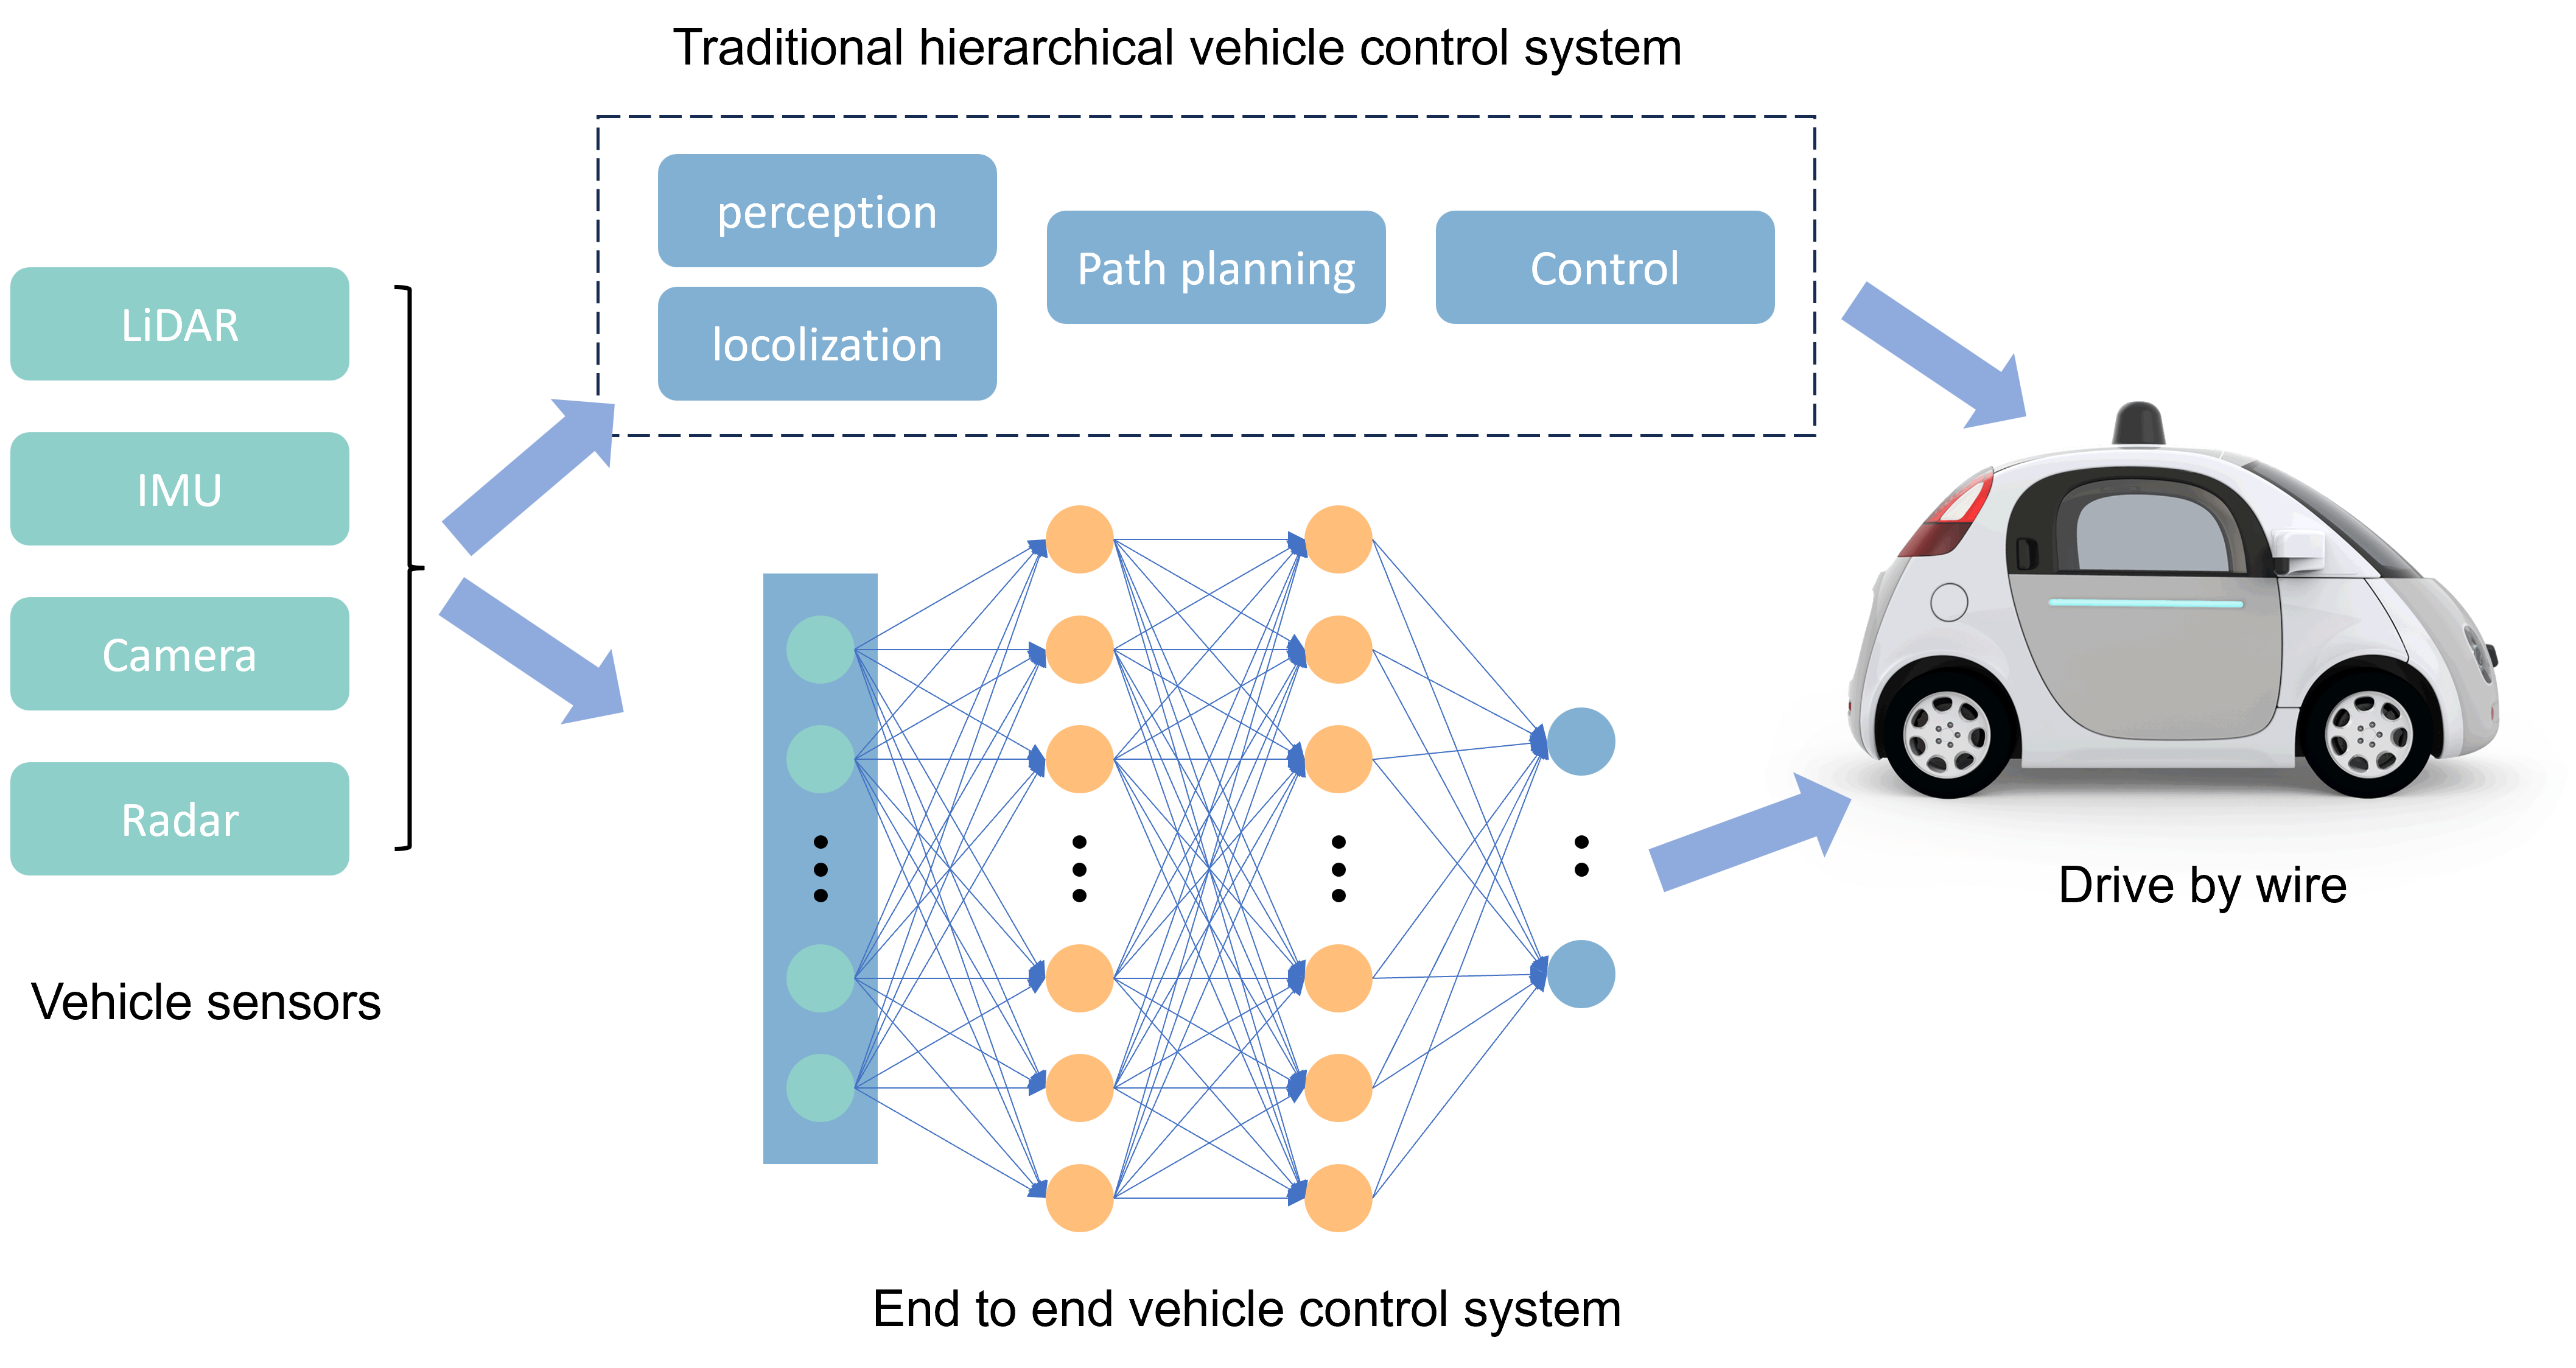
\includegraphics{fig/traditional_endToEnd.png}}
\caption{Comparison between traditional hierarchical vehicle control system and end to end vehicle control system}
\label{fig: traditional endToEnd}
\end{figure}

In the realm of end-to-end autonomous driving, various research methods have been employed to achieve seamless control and navigation. The work from Nvidia by using a Convolutional Neural Network to directly map raw pixels from cameras to steering commands has been a foundational approach, simplifying the control process by directly linking visual input to driving actions. Building on this, Imitation Learning (IL), or learning from demonstrations, has emerged as a technique where an agent learns the optimal policy by imitating expert human behavior, providing a data-driven way to capture complex driving strategies. Reinforcement learning has extend this idea further by mapping raw pixels to discretized actions, offering a more interactive and self improving control mechanism, which demonstrated successful results on real world driving recently, including lane following \parencite{kendall2019learning} and urban driving \parencite{jaritz2018end}. Peng et al \parencite{peng2021end} introduces an end-to-end autonomous driving approach utilizing the Dueling Double Deep Q-Network, a deep reinforcement learning algorithm. This method enables the vehicle to independently learn end-to-end driving, fostering self-reliance in navigation and control. Actor-Critic Methods, such as A3C, DDPG, and TD3, have been applied to handle complex decision-making and planning problems, integrating both value and policy-based learning for more robust control. Reinforcement learning has been successfully applied in autonomous driving when combined with supervised learning in recent years. The future of RL in autonomous driving faces challenges in transferring findings from simulation to the real world. Simplistic reward functions may encourage risky behavior \parencite{knox2023reward}, and designing or learning better functions remains an open problem. Combining RL with world models and enhancing representation learning are key areas for ongoing exploration and development. Also, current RL solutions for autonomous driving will be hindered by high dimensional representation due to computational cost, and research is still on going for the model to learn from and interact with the world in a more data efficient way \parencite{chen2023end}.

In conclusion, the end-to-end autonomous driving using Deep Reinforcement Learning has emerged as a promising direction, offering simplicity, adaptability, and the potential for superior performance. It stands in contrast to traditional hierarchical methods, providing a more integrated and flexible approach. However, challenges related to data dependency, interpretability, sensor integration, and robustness continue to be areas of active research and development. The ongoing exploration of various DRL algorithms, combined with real-world training and attention to interpretability, is shaping the future of autonomous driving, making it an exciting and dynamic field of study.

\section{Model based reinforcement learning in autonomous driving}

In reinforcement learning context, unlike other machine learning methods, the learning process is pushed forward using the interactions between the agent and the environment, which means the agent learns control mapping function directly from its surroundings without requiring supervision. However, discrimination between the agent and the environment is not always clear, which varies in different application. For instance, in autonomous driving problems, the vehicle's actuator response are often considered part of the environment.

The main difference between model-based and model free reinforcement learning is whether a model of the interactions between the robot and the environment is employed. MFRL algorithm learns the control policy without such model, and instead, it relies on the method called trial-and-error, which directly with the physical system to discern rewards and determine optimal actions. On the other hand, MBRL incorporates a model which captures the environment transition dynamics, and use this model as the foundation for reward determination and action optimization. Consequently, in model-based approaches, policies are fine-tuned using the model, and once optimized, they are then deployed on the actual system. This process is depicted in Figure \ref{fig: mbrl schema.png}, and shows the typical data flow of a model-based reinforcement learning approach.

\begin{figure}[h]
    \centering
    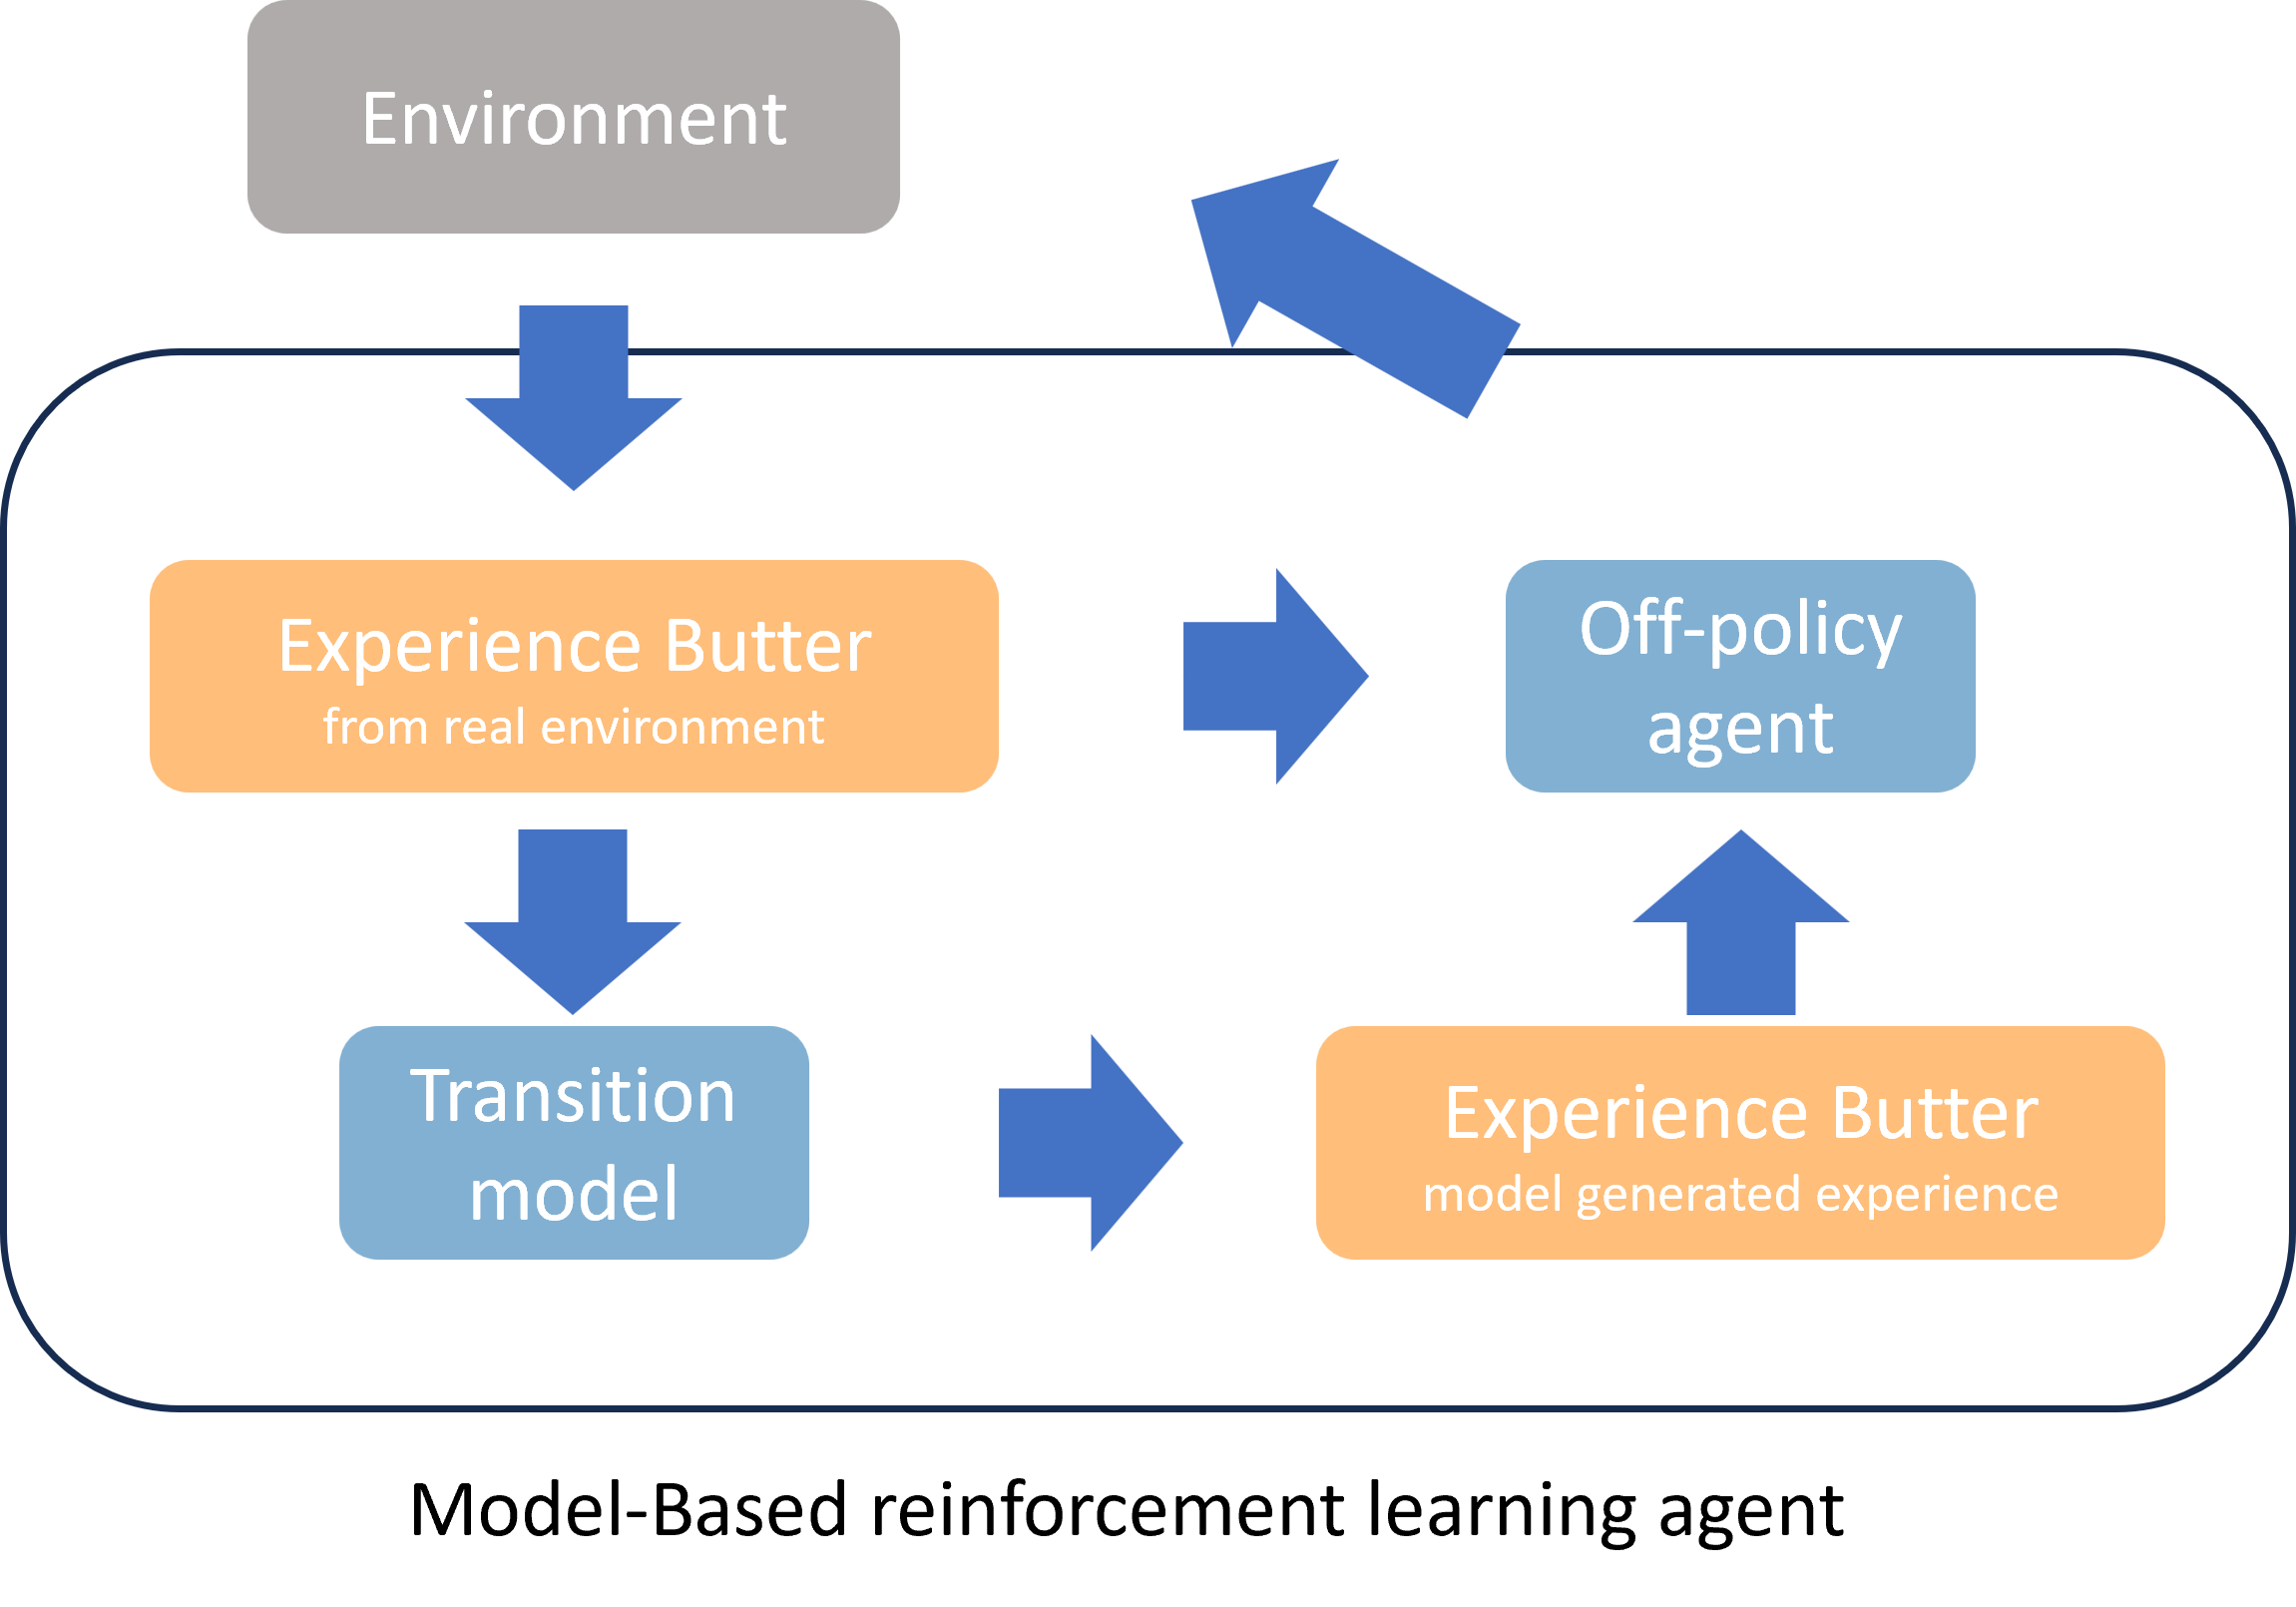
\includegraphics[width=0.7\textwidth]{fig/mbrl schema.png}
    \caption{Model-based reinforcement learning schema}
    \label{fig: mbrl schema.png}
\end{figure}

Nowadays, the model-based reinforcement learning has been proven to be sampling efficiency and wide adaptable in the field of robotics. Huang et. al. investigated the challenge of parametrizing
policies for reinforcement learning in highdimensional continuous action spaces, and present a practical model-based RL method leverages the multimodal policy parameterization and learned world model to achieve strong exploration capabilities and high data efficiency \parencite{huang2023reparameterized}. Hu et. al. introduces a model-based reinforcement learning technique for autonomous driving, which learns the world model and driving policy using 3D geometry from high-resolution expert videos. Trained offline on urban driving data, MILE outperforms previous methods by $31\%$ in the CARLA simulator under new conditions. It uniquely integrates static and dynamic scene modeling with ego-behavior using only cameras\parencite{hu2022model}. Heess et. al. introduced a unified framework for learning continuous control policies via backpropagation, developed multiple RL algorithms based on teh framework, and then compared the general policy gradient algorithms that range from model-free methods with value functions to model-based methods without value functions. The results showed that the model-based algorithm SVG(1) shows the effectiveness of learning models, value functions, and policies simultaneously in continuous domains comapred with other competators. 

To conclude, model-based reinforcement learning is becoming a popular research area as it requires fewer interactions with the environment compared to model-free RL, which reduced interaction not only minimizes the risk of accidents but also reduces wear and tear on the robot. To successfully implement MBRL, the transition models should be designed carefully, which will affect the performance of the learning algorithm in terms of accuracy and convergence. Furthermore, imitation learning combined with RL, by guided by human demonstrations, making RL a promising approach for tasks like autonomous driving where human-like decision-making is preferred.